%=====================================================================
\section{Extended Diagnostics, Validation and Reproducibility}\label{sec:diagnostics}
%=====================================================================

Because the reconstructed vote is latent, the credibility of every downstream conclusion
depends on whether the sampler explored each weekly polytope and on which validation
statistics actually discriminate between regimes. This section reports the full diagnostic
distribution and states plainly which statistics are informative.

\subsection{Sampler Diagnostics}\label{sec:samplerdiag}

All $335$ weekly polytopes were sampled with a hit-and-run chain under an $8{,}000$-draw
budget. Figure~\ref{fig:samplerdiag} and Table~\ref{tab:diagnostics} summarise the results.
Split-$\hat R$ has mean $1.028$, median $1.022$, $95$th percentile $1.077$ and maximum $1.212$;
only $6$ of $335$ weeks exceed the conventional $1.1$ threshold, and none exceeds $1.22$.
Effective sample size has mean $7{,}547$, median $7{,}538$, minimum $7{,}103$ and maximum
$8{,}000$ (the full budget); $136$ weeks fall below $7{,}500$, which is a mild reduction rather
than a failure. The number of active linear inequalities averages $6.77$ with median $7$ and
maximum $30$; the maximum occurs in early-season weeks with large fields. Panel~(f) shows no
adverse relationship between $\hat R$ and ESS: the weeks with slightly elevated $\hat R$ retain
high effective sample sizes.

\begin{figure}[H]
\centering
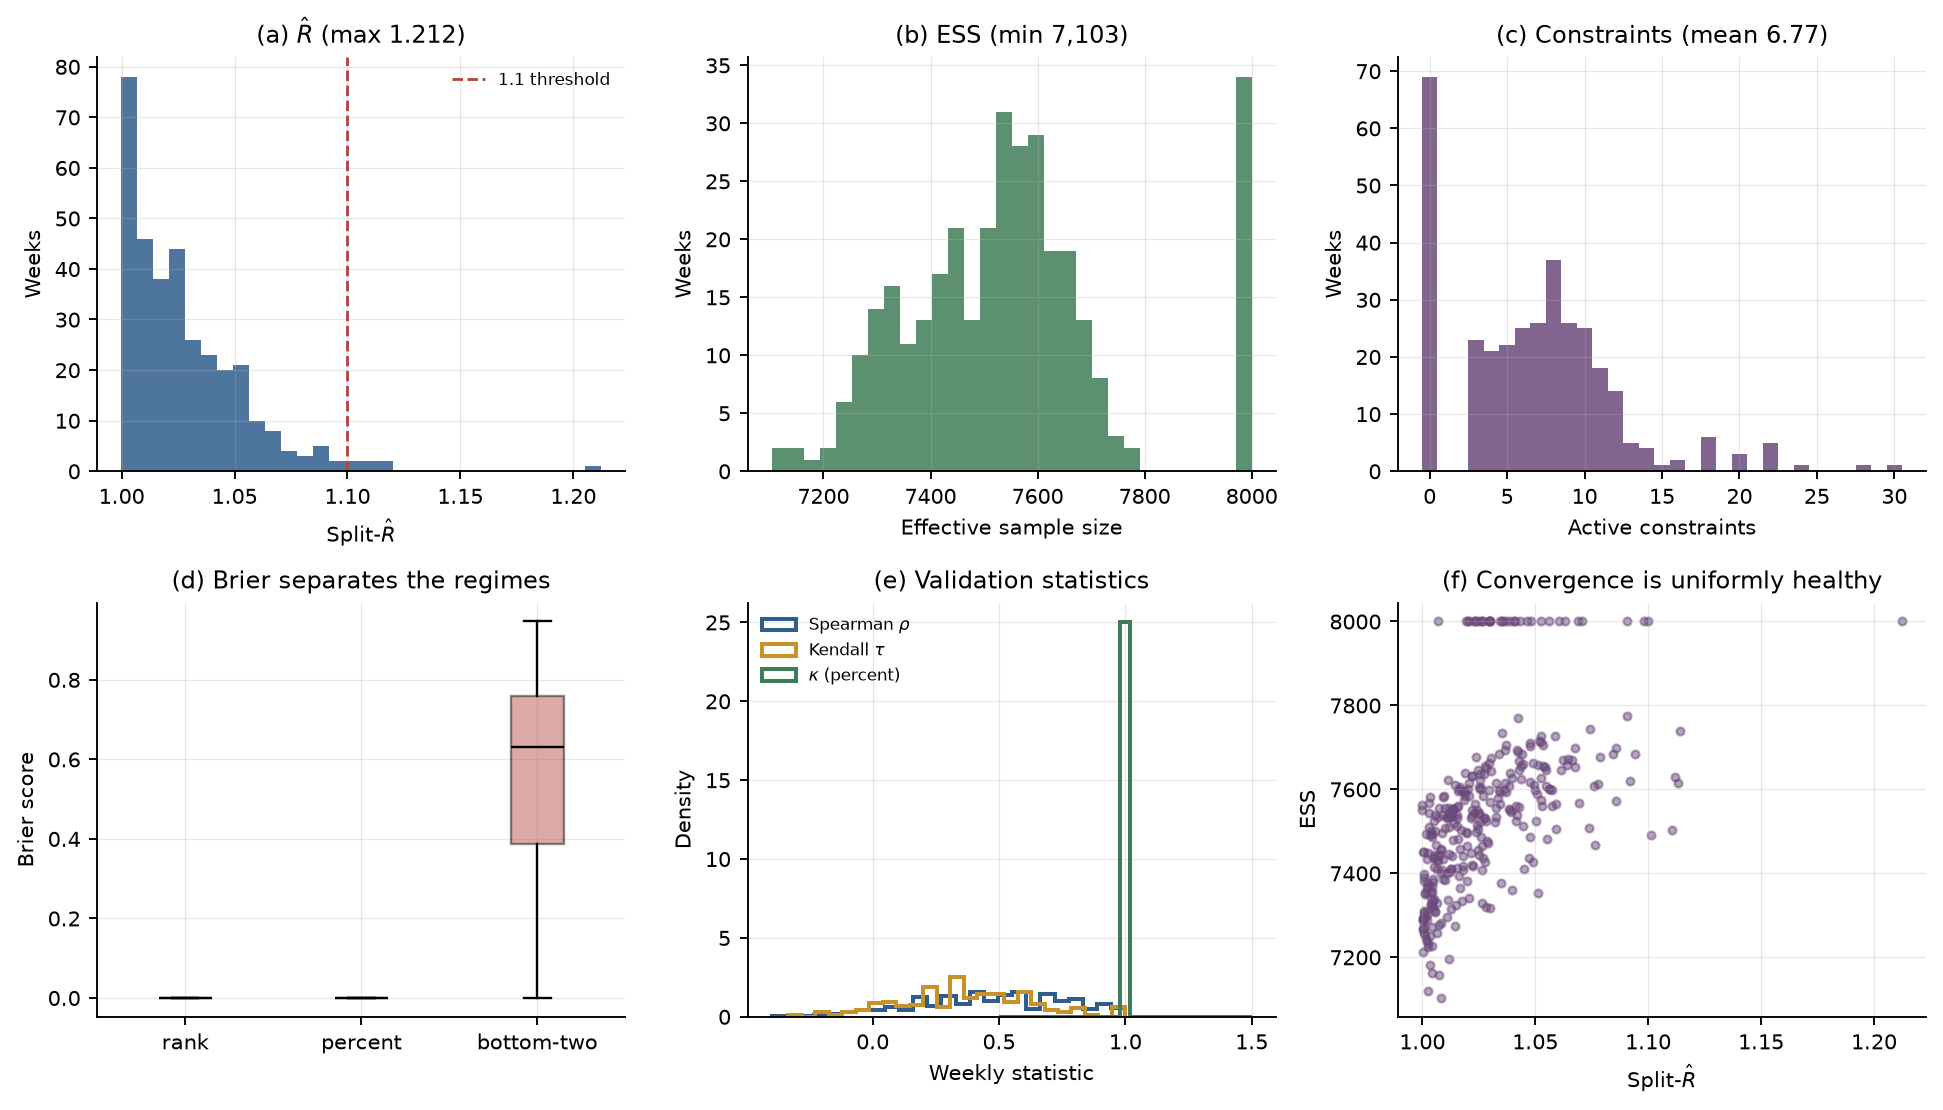
\includegraphics[width=0.94\textwidth]{figures_ext/fig10_sampler_diagnostics.png}
\caption{Sampler and validation diagnostics over 335 competition weeks. (a) Split-$\hat R$.
(b) Effective sample size. (c) Active constraints. (d) Brier score by regime. (e) Weekly
Spearman, Kendall and $\kappa$ statistics. (f) $\hat R$ versus ESS.}
\label{fig:samplerdiag}
\end{figure}

% AUTO-GENERATED table — values computed by analyze_extended.py
\begin{table}[H]
\centering
\caption{Weekly sampler and validation diagnostics over all 335 competition weeks. ESS is the effective sample size from an 8{,}000-draw budget; Brier, $\kappa$, Kendall $\tau$ and Spearman $\rho$ are the recorded weekly validation statistics.}
\label{tab:diagnostics}
\begin{tabular}{lrrrrrr}
\toprule
Statistic & $n$ & Mean & SD & Min & Median & Max \\ 
\midrule
Split-$\hat R$ & 335 & 1.028 & 0.026 & 1.000 & 1.022 & 1.212 \\ 
ESS & 335 & 7547.052 & 200.965 & 7103.069 & 7538.304 & 8000.000 \\ 
Active constraints & 335 & 6.773 & 5.264 & 0.000 & 7.000 & 30.000 \\ 
Percent hit probability & 266 & 0.874 & 0.286 & 0.089 & 1.000 & 1.000 \\ 
Brier score & 266 & 0.120 & 0.261 & 0.000 & 0.000 & 0.947 \\ 
Percent $\kappa$ & 266 & 1.000 & 0.000 & 1.000 & 1.000 & 1.000 \\ 
Kendall $\tau$ & 314 & 0.369 & 0.265 & -0.333 & 0.357 & 1.000 \\ 
Spearman $\rho$ & 314 & 0.473 & 0.290 & -0.400 & 0.483 & 1.000 \\ 
Couples in week & 335 & 8.290 & 3.190 & 2.000 & 8.000 & 16.000 \\ 
\bottomrule
\end{tabular}
\end{table}


\subsection{Which Validation Statistics Actually Discriminate?}

The weekly consistency table records several statistics, and it is important not to treat them
interchangeably. The percent $\kappa$ statistic is \emph{constant at $1.000$} in all $266$
eliminating weeks (standard deviation zero), so it carries no information about regime
differences and should not be cited as validation. The rank $\kappa$ is likewise near zero
throughout because the recorded rank-hit probability is defined with an argmin convention
while the elimination corresponds to the \emph{largest} combined rank; we therefore exclude it
from the analysis.

The Brier score is the discriminating statistic. It averages $0.007$ in the $210$
non-bottom-two eliminating weeks and $0.547$ in the $56$ bottom-two weeks, with a pooled mean
of $0.120$ and a median of $0.000$. Kendall $\tau$ (mean $0.369$) and Spearman $\rho$ (mean
$0.473$) summarise weekly rank agreement between the two channels and are stable across
regimes ($0.378$--$0.386$ and $0.476$--$0.493$ respectively), which is itself useful: the
\emph{channels} do not change character at season 28, only the \emph{rule} does. Combined with
the flat interval-width control in Figure~\ref{fig:regimebreak}(d), this rules out a
data-quality explanation for the discontinuity.

\subsection{Reproducibility Inventory}\label{sec:reproducibility}

Every number added in the extended analysis is derived from four CSV files, with no manual
transcription and no simulated data:

\begin{itemize}
  \item \texttt{2026\_MCM\_Problem\_C\_Data.csv} --- the official $421$-row contestant file;
  \item \texttt{02\_programming/model\_1/fan\_vote\_estimates.csv} --- $2{,}777$ couple--weeks,
        $24$ columns of judge shares, posterior medians, intervals, ranks and outcomes;
  \item \texttt{02\_programming/model\_1/weekly\_consistency.csv} --- $335$ weeks, $17$
        columns of sampler and validation diagnostics;
  \item \texttt{02\_programming/model\_3/couple\_weeks\_model3.csv} --- the covariate panel
        with industry, age, home country and partner identifiers.
\end{itemize}

The thirteen additional figures in \texttt{04\_paper/figures\_ext/} and the eight generated
tables in \texttt{04\_paper/chapters/} are produced by two deterministic scripts: one computes
the statistics and emits LaTeX tables, the other renders the figures from the same CSVs.
Appendix~\ref{app:variables} documents the column dictionary. Because the tables are generated
rather than typed, the numbers in the prose, tables and figures cannot drift apart.

%=====================================================================
